\documentclass{beamer}
\mode<presentation>
{
  \usetheme{default}      % or try Darmstadt, Madrid, Warsaw, ...
  \usecolortheme{default} % or try albatross, beaver, crane, ...
  \usefonttheme{default}  % or try serif, structurebold, ...
  \setbeamertemplate{navigation symbols}{}
  \setbeamertemplate{caption}[numbered]
} 

\usepackage[english]{babel}
\usepackage[utf8]{inputenc}
\usepackage[T1]{fontenc}
\usepackage{amssymb}
\usepackage{amsmath}
\usepackage[T1]{fontenc}
\usepackage{subfigure}
\usepackage{graphicx}


\title[Your Short Title]{EE2227 Control Systems}
\author{EE18BTECH11050}
\institute{Krati Arela}
\date{February 16,2020}

\begin{document}

\begin{frame}
  \titlepage
\end{frame}

\section{Introduction}

\begin{frame}{Question 20/GATE EC-2015}


\begin{block}{Question}
A unity negative feedback system has the open loop transfer function\newline
\[G(s) = \frac{K}{s(s+1)(s+3)}\]\newline
The value of the gain K (>0) at which the root locus crosses the imaginary axis is ?
\end{block}

\end{frame}

\section{Solution}

\begin{frame}{Root Locus}
\begin{itemize}
\item The Root locus is the locus of the roots of the characteristic equation, which are the poles of closed loop transfer function, by varying system gain K from $0$ to $\infty$.

\item The characteristic equation of the closed loop control system is: 
\[1 + G(s)H(s) = 0\]
\item The points on the root locus branches must satisfy the \textbf{angle condition.}
\item We can find the value of K for the points on the root locus branches by using \textbf{magnitude condition.}
\end{itemize}
\end{frame}

\begin{frame}{Conditions for Root Locus}

\begin{itemize}
    \item Angle Condition:
    Given the Characteristic equation:
    \[1+G(s)H(s) = 0\]
    $\implies$\[G(s)H(s) = -1 + j0\]
    The phase angle of G(s)H(s) is:
    $\angle$G(s)H(s) =\[ \arctan(\frac{0}{-1}) = (2n+1)\pi\]
    \item The angle condition is the point at which the angle of the transfer function is an odd multiple of 180.
\end{itemize}

\end{frame}

\begin{frame}{Conditions for Root Locus}

\begin{itemize}
    \item Magnitude Condition:
    Magnitude of G(s)H(s) is:
    \[|G(s)H(s)| = \sqrt{(-1)^2 + 0^2}\]
    $\implies$\[|G(s)H(s)| =1 \]
    \item The magnitude condition is that the point (which satisfied the angle condition) at which the magnitude of the transfer function is one.
\end{itemize}

\end{frame}

\begin{frame}{Root Locus Examples}

\begin{figure}
    \centering
    \begin{subfigure}
        
        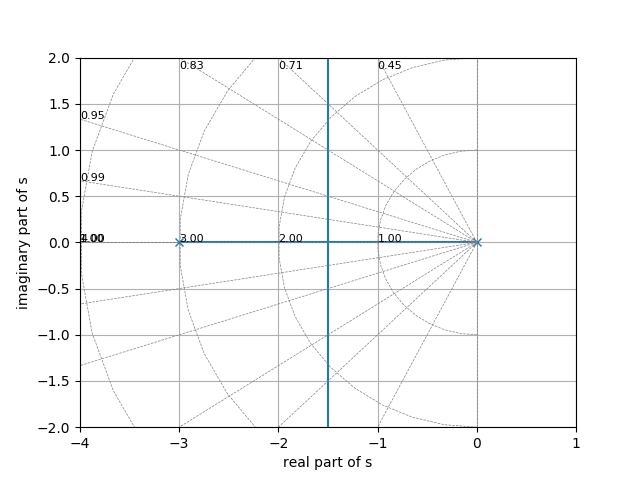
\includegraphics[width=120 pt]{rl1.png}
        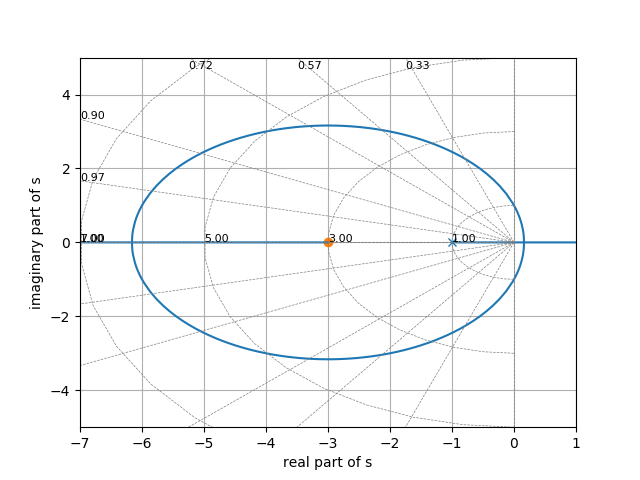
\includegraphics[width=120 pt]{rl2.png}

    \end{subfigure}
    \begin{subfigure}
        
        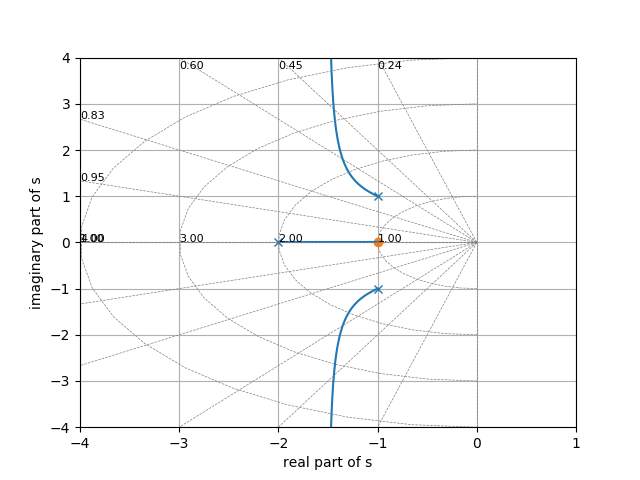
\includegraphics[width=120 pt]{rl3.png}
        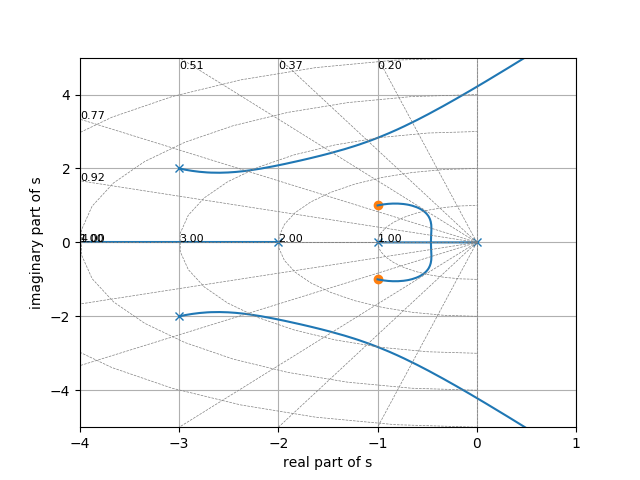
\includegraphics[width=120 pt]{rl4.png}

    \end{subfigure}
\end{figure}
    
\end{frame}

\begin{frame}{Solution}
Given open loop transfer function\newline
\[G(s) = \frac{K}{s(s+1)(s+3)}\]\newline
we have P = 3 poles, at s = 0,-1,-3 and Z = 0 zeroes.
\newline
\newline
For unity negative feedback, closed loop transfer function is:\newline
\[T(s)= \frac{G(s)H(s)}{1+G(s)H(s)}\]\newline

Here H(s) = 1\newline
$\implies$\[T(s) = \frac{K}{s(s+1)(s+3)+K}\]

\end{frame}

\begin{frame}{Solution}

Poles of closed loop transfer function are the roots of the Characteristic Equation.\newline
Given characteristic Equation is:
\newline
\[ 1 + G(s)H(s) = 0\]\newline
$\implies$ \[ s^3 + 4s^2 + 3s + K = 0\] \newline

\textbf{If all elements of any row of the Routh array table are zero, then the root locus branch intersects the imaginary axis}\newline
\end{frame}

\begin{frame}{Solution}
Routh Array Table:\newline
\begin{table}
\centering
\begin{tabular}{l|r r}
Order & Coefficients\\\hline
$s^3$ & 1 & 3 \\
$s^2$ & 4 & K \\
$s^1$ & (12-K)/4 & 0\\
$s^0$ & K & 
\end{tabular}

\end{table}

For poles to be on imaginary axis, row $s^1$ should be zero.\newline
So, \[\frac{12-K}{4} = 0\]
\newline Hence, $$\textbf{K = 12}$$


\end{frame}

\begin{frame}{Verification}
Auxilliary equation:
\[4s^2 + K = 0\]
$\implies$ \[ 4s^2 + 12 = 0\] 
$\implies$ \[ s = -j\sqrt{3},+j\sqrt{3} \] \newline
Thus a pair of poles lie on imaginary axis for K = 12.


\end{frame}


\begin{frame}{Plot}
\begin{figure}
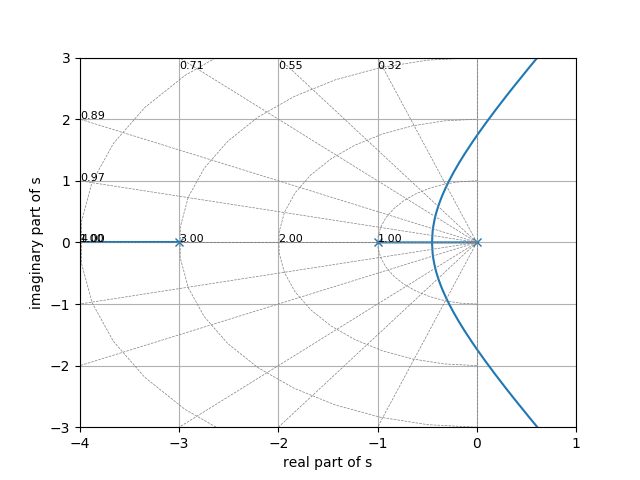
\includegraphics[width=250 pt]{Root_Locus.png}
\caption{\label{fig:your-figure}Root Locus Plot}
\end{figure}


\end{frame}

\end{document}

